\documentclass[11pt]{article}
\usepackage{graphicx}
\usepackage{amsmath,amsthm,amsfonts}
\usepackage{epsfig,graphics}
\usepackage{hyperref}
\usepackage{verbatim}
\usepackage{mathrsfs}
\usepackage{xcolor}

\setlength{\textheight}{8.5in}
\setlength{\evensidemargin}{0.0in}
\setlength{\oddsidemargin}{0.0in}
\setlength{\topmargin}{-0.5in}
\setlength{\textwidth}{6.5in}

\newtheorem{theorem}{Theorem}
\newtheorem*{theorem*}{Theorem}
\newtheorem{claim}{Claim}
\newtheorem*{claim*}{Claim}
\newtheorem{lemma}{Lemma}
\newtheorem*{lemma*}{Lemma}
\newtheorem{proposition}{Proposition}
\newtheorem*{proposition*}{proposition}
\newtheorem{exercise}{Exercise}
\newtheorem*{exercise*}{Exercise}
\newtheorem{corollary}{Corollary}
\theoremstyle{definition}
\newtheorem{definition}{Definition}
\newtheorem{fact}{Fact}
\newtheorem*{fact*}{Fact}



\newcommand{\handout}[6]{
   \renewcommand{\thepage}{#1-\arabic{page}}
   \noindent
   \begin{center}
      \vbox{
    \hbox to \textwidth { #2 \hfill #3 }
       \vspace{4mm}
       \hbox to \textwidth { {\Large \hfill #4  \hfill} }
       \vspace{2mm}
       \hbox to \textwidth { { #5 \hfill #6} }
      }
   \hrulefill
   \end{center}
   \vspace*{4mm}
}

%\newcommand{\lecture}[5]{\handout{#1}{#2}{#3}{#4}{#5}}


% Types of Variables
\newcommand{\bvar}[1]{\mathbf{#1}} % bold variable
\newcommand{\mvar}[1]{\bvar{#1}} % matrix variable
\newcommand{\vvar}[1]{\vec{#1}} % vector variable

% Domains
\newcommand{\R}{\mathbb{R}}
\newcommand{\Z}{\mathbb{Z}}
\newcommand{\redgevec}{\R^{E}}
\newcommand{\rvertvec}{\R^{V}}
\newcommand{\rPos}{\R^{+}}
\newcommand{\rNonNeg}{\R^{\geq 0}}

% Symbol for definitions
\newcommand{\defeq}{\stackrel{\mathrm{\scriptscriptstyle def}}{=}}

% Optimization
\DeclareMathOperator*{\argmin}{arg\,min}
\DeclareMathOperator{\Cone}{Cone}
\DeclareMathOperator{\Cut}{CUT}

% Types of Graphs
\newcommand{\nlap}{\mathscr{L}_G}
\newcommand{\pseudo}[1]{{#1}^\dagger}
\newcommand{\lapPseudo}{\pseudo{\lap}}
\newcommand{\adj}{A}
\newcommand{\incMatrix}{\mvar{B}}
\newcommand{\diag}{\operatorname{diag}}
\newcommand{\rMatrix}{\mvar{R}} % resistance matrix
\newcommand{\iMatrix}{\mvar{I}} % identity matrix
\newcommand{\Vol}{\textrm{Vol}}


% Vectors
\newcommand{\1}{\vec{1}}
\renewcommand{\dot}[1]{\langle {#1} \rangle}

%other
\DeclareMathOperator{\sgn}{sgn}



\begin{document}

\handout{}{CS 591 O1: Iterative Methods for Graph Algorithms and Network Analysis}{Fall 2018}{Lecture 2: Linear Algebra Review}{Instructor: Lorenzo Orecchia}{Scribe: Lorenzo Orecchia}

\section{The Computer Science way}

In Computer Science, Spectral Graph Theory is usually introduced by equating graphs with matrices\cite{chungSpectralGraphTheory,spielmanSpectralGraphTheory2007}. 
% LONOTE: IMPROVE THIS SENTENCE. ADD REFERENCES...

\paragraph{Undirected Graphs}
Unless explicitly stated, all graphs that we will deal with in this part of the course are undirected graphs, i.e. the edges are unordered pairs of vertices and have no direction. They will also be loopless and simple (no multiple edges).
%
A (weighted) undirected graph is formally described as a tuple $G = (V, E, \vw \in \R_{>0}^E),$ where $V$ is a set of vertices, $E \subseteq V \times V$ is a collection of edges, i.e. unordered pairs of vertices from $V$ and $\vw$ are the associated positive weights.
%
The graph is unweighted if  $\vw = \mathbf{1}$.
%In that case we will describe a graph as a pair $G = (V, E)$.
%
As we only consider finite graphs, we can assume without loss of generality that $V = [n] = \{i \in \mathbb{N}: 1 \leq i \leq n\},$ for some integer $n \geq 1.$
%

These assumptions may seem restrictive, but they are exactly what is needed for modeling interactions between pairs of vertices where the weight may represent the strength of the interaction. For instance, the weights of the edges may represent a measure of similarity between their endpoints, as in similarity-based learning.
%
The main reason why we want to limit ourselves to undirected graphs is that they can naturally be represented as {\it symmetric} square matrices. 

\paragraph{The Adjacency Matrix} The first graph matrix we introduce is the most intuitive representation of an undirected graph.
\begin{definition}
The adjacency matrix $\mA_G$ of a graph $G=(V,E, \vw)$ is a $n \times n$ square matrix with
$$
(\mA_G)_ {ij} = 
							\begin{cases}
							w_{ij}, \enspace \{i,j\} \in E \\
							0,       \enspace \textrm{otherwise}
							\end{cases}
$$
\end{definition}
It should be clear by the undirectedness of $G$ that $\mA_G$ is symmetric.
%
While the adjacency matrix is a simple way of defining a graph matrix, it turns out that a normalized version of the adjacency defines a more natural operator of $\R^n:$ the random walk operator. To define this operator, we first need to introduce an auxiliary graph matrix, the degree matrix.

\paragraph{The Degree Matrix}

Recall that the degree $d_i$ of a vertex $i \in V$ for a weighted graph $G=(V,E, w)$ is defined as $d_i \defeq \sum_{\{i,j\} \in E} w_{ij}.$ The degree distribution will often be the natural measure over the vertices of the graph. For this reason, it is convenient to have a diagonal matrix representing degrees.
\begin{definition}
The degree matrix ${D}_G$ of $G=(V,E, w)$ is  the diagonal matrix such that, for all $i \in [n]$
$$
({\mD}_G)_{ii} = d_i = \sum_{\{i,j\} \in E} w_{ij}.
$$ 
\end{definition}
A quick observation: when the graph $G$ is regular, i.e., all degrees are equal to some $d,$ then the degree matrix is just a multiple of the identity, $\mD_G = d \mI.$ For the rest of the course, we will omit the subscript indicating the graph $G$ when the context is clear.

\subsection{Natural Random Walk on $G$} \label{sec:random-walk}

\paragraph{The Natural Random Walk and Its Matrix}
Consider a particle moving in a random fashion over the vertices $V$ of the graph $G$ and transitioning from vertex to vertex at discrete time intervals. Let $X(t) \in V$ be a random variable describing the position of the particle at time $t \in \Z.$ The weights on the edges of $G$ regulate the random transitions of $X(t)$ as follows: suppose that at time $t$ the particle is at vertex $v$, that is $X(t) = v$. At time $t+1,$ the particle randomly picks an incident edge $\{u,v\}$, with probability proportional to its weight $w_{uv}.$ It then moves to the other end of the edge,i.e., $X(t+1)$ = u. Formally:
\begin{equation} \label{eq:mc}
\Pr[X(t+1) = u | X(t) = v] = \begin{cases}
    \frac{w_{uv}}{d_v}, \enspace \{u,v\} \in E\\
    0, \enspace \textrm{ow}.
\end{cases}
\end{equation}
We refer to this discrete-time Markov chain as the {\it natural random walk over the graph}. 
%
Let  $\vp^{(t)} \in \mathbb{R}^n_{\geq 0}$ be a vector describing the probability distribution of $X(t)$ over the vertices of the graph. By Equation~\ref{eq:mc}, we can compute the evolution of $p^{(t)}$ as follows:
\begin{equation}
p^{(t+1)}_i = \sum_{\{i,j\} \in E} \Pr\{X_{t+1} = i | X_{t} = j \} \Pr\{X_{t} = j\} = \sum_{\{i,j\} \in E}
\frac{w_{ij}}{d_j} \cdot p^{(t)}_j = ({\mA} \mD^{-1} \vp^{(t)})_i.
\end{equation}
In words,  when we apply one step of the random walk the amount of probability mass at $i$  is the sum of all the contributions from neighbors of $i.$ 


%%% LONOTE: example of a natural process captured by this


\begin{definition}
The random walk matrix $\mP_G$ of $G=(V,E,w)$ is defined as
$$
{\mP_G} = {\mA}_G {\mD}_G^{-1}
$$
\end{definition}
Formally, the random walk matrix $\mW_G$ is also the transition probability matrix for the Markov chain $X(t)$. 
%
%In words, the random walk matrix ${W}_G$ describes the transition probabilities of the random process and allows us to keep track of the {\it marginal probability} that the random walk is at a certain node.
Note that there is nothing random about ${W}_G$. It just helps in describing the probability distributions arising from the random walk process.



\paragraph{The Laplacian Matrix} The random walk matrix described a natural process, but it is unfortunately not symmetric in general, unless the graph is regular. A related symmetric matrix that turns out to be the most useful for Spectral Graph Theory is the Laplacian matrix. Here is one definition of the Laplacian. We will see another in the next chapter.

\begin{definition} \label{def:laplacian}
The Laplacian matrix $\mL_G$ of $G=(V,E,\vw)$ is the matrix $\mL_G \defeq \mD_G - \mA_G.$ Equivalently:
$$
(\mL_G)_ {ij}= 
							\begin{cases}
							d_i, \enspace i=j\\
							-w_{ij}, \enspace \{i,j\} \in E \\
							0,       \enspace \textrm{otherwise}
							\end{cases}
$$
\end{definition}

\paragraph{Next Steps}
The next steps in the standard CS development of the subject is to apply the spectral theorem to the symmetric matrix $\mL_G$ to understand the behavior of $\mP^t_G$ by exploiting the relation
$$
\mP_G = \mI - \mL_G \mD_G^{-1}.
$$
By contrast, in this course, we will discuss more in depth how the Laplacian matrix arises as a discrete analogue of the Laplacian differential operator over the space of functions on a continuous domain, such as a manifold. 

\section{The Partial Differential Equations (PDE) way}

Historically, spectral methods were developed in the late 1970s to solve certain families of smooth partial differential equations over $\R^n.$
%
Indeed, throughout the course, we will often use the same techniques to analyse and implement solvers for the discrete analogues of these PDEs. 
%
Because I believe that the continuous pictures, albeit mathematically harder to formulate, reveals some important intuition about spectral methods over graphs, in this section I will try to introduce and motivate the basic operators in spectral graph theory via an informal discussion of their continuous counterparts. A great reference for all continuous instances of the Laplacian operator is the book ``The Laplacian on a Riemannian Manifold'' by Rosenberg~\cite{rosenbergLaplacianRiemannianManifold1997}.

\subsection{The Laplacian $\Delta$ over Compact Subsets of $\R^n$}


% LONOTE: check this part. should we use L_2 instead?

We will define the Laplacian $\Delta$ as the second-order differential operator  defined by:
$$
\left(\Delta f\right)\left(\vx_0\right) =
- \sum_{i=1}^{n} \frac{\partial^2 f}{\partial x_i^2}\Big|_{\vx_0} = 
- \nabla \cdot \nabla f 
= 
-\text{div}\left(\nabla f\right)\left(\vx_0\right)
$$
Even though this can be defined for any twice-differentiable function over $\R^n,$ for this discussion it will be easier to consider the action of $\Delta$ 
over the space $C^\infty_{0}([0,1]^n)$, i.e., smooth functions over $[0,1]^n$ that vanish on the boundary.
%
Notice that $\Delta$ acts as a linear operator over this space, taking in $f \in C^\infty_{0}([0,1]^n)$ and returning another function $\Delta f$ in the same vector space of functions. We can also equip this space with the following natural notion of inner product:
$$
\langle f, g \rangle =  \int_{[0,1]^n} f(\vx) g(\vx) d\vx.
$$
This allows us to define a notion of adjoint, i.e. a generalization of the transpose, for the linear operator $\Delta$. By applying integration by parts twice and exploiting the compactness of the support of $f$ and $g$, we find that:
$$
\langle \Delta f, g \rangle =  \langle \nabla f, \nabla g \rangle = \langle f, \Delta g \rangle. 
$$
This shows that the linear operator $\Delta$ is a self-adjoint operator, the infinite-dimensional analogue of a symmetric matrix. Hence, we may expect $\Delta$ to exhibit an analogue to an orthonormal basis of eigenvectors. Indeed, such a basis is given by the cosine functions 
$
\{\cos(2\pi \; \vlambda \cdot \vx)\}_{\vlambda \in \Z^n},
$
which are just the real part of the Fourier basis functions.
%
It is not hard to compute the corresponding eigenvalues:
$$
(\Delta \cos(2\pi \; \vlambda \cdot \vx))(x_0) = - \|\vlambda\|^2 \cdot \cos(2\pi \; \vlambda \cdot \vx).
$$
It is possible to extend this reasoning to more interesting function spaces such as functions over $\R^n$, where the orthonormal systems yields the Fourier transform. However, the correct choice of function space for this piece of math to work is fairly complex (see Rigged Hilbert Space). 
% see Rosenberg

\paragraph{Applications of the Laplacian}

The Laplacian is used in three very important PDEs. Three out of four fundamental PDEs in Chapter \cite{evansPartialDifferentialEquations2022} Evans's standard PDE textbook involve the Laplacian. They are:
\begin{itemize}
    \item {\bf Laplace's equation} describes the steady state in a field
    $$\Delta f = 0$$

    \item {\bf Heat equation} connects the time derivative to the spatial gradient. Given a function $f^{(t)}: [0, \infty) \times \R^n$
    $$\frac{d f}{dt} = - \Delta f$$

    \item {\bf Wave equation} describes a standing wave
    $$\frac{d^2 f}{dt^2} = -\Delta f$$
\end{itemize}

What makes the Laplacian such an ubiquitous object in these models of natural phenomena? To answer this question, it is helpful to visualize the interpretation of the Laplacian as the divergence of the gradient of a function (or potential) $f$. You may equivalently think of $f(\vx)$ as a temperature or the concentration of a substance at $\vx.$
%ELECTRIC FIELD? CHECK
%EXAMPLE SOMEWHERE, NOT IN EVANS
This difference in temperature (or concentration) leads to a flow of heat (or of the substance) from high temperature to low temperature regions.
This takes the form of a vector field $-\nabla f(\vx)$. When flows moves along this vector field, the net in-flux at a point $\vx$ is given by the negative divergence of $-\nabla f(\vx).$  Combining these two facts, the change in temperature at $\vx$ becomes:
$$
\frac{df}{dt}(\vx) = (-\operatorname{div})(-\nabla f(\vx)) = - (\Delta f)(\vx).
$$

\paragraph{Generalized Laplacian} We can slightly generalize the notion of Laplacian by introduce a notion of conductivity $w(\vx)$ at each point. The flow of heat at $\vx$ takes now the form $-w(\vx) \nabla f(\vx)$ and the resulting Laplacian is:
$$
\Delta_w(f) = -\operatorname{div}(w \cdot \nabla f).
$$

% HERE: add different heat conductivty 

% FLUX vs FLOW
% CITATION FOR DERIVATION OF LAPLACIAN
% LONOTE: different forms of Laplacians
%LONOTE: see Rosenberg
%IMAGE FOR THIS

\subsection{Graph Discretization} 

From this perspective, spectral graph theory naturally arises when discretizing the continuous space into a graph with edges connecting neighboring centers, with the caveat that typical discretizations of physical phenomena involve grids or meshes that are good representation of physical space, while general spectral algorithms often involve graphs, such as the Web graphs, that do not have natural low-dimensional representations. We now derive a few more graph matrices based on discretizing the continuous differential operators in the discussion above. In particular, we will be interested in discrete analogue of the gradient operator $\nabla$ and the divergence operator $\operatorname{div}.$



\paragraph{Gradient Operator}
Given a vector field $\vx \in \R^V$ we would like the equivalent to the gradient operator.
%
This operator should return flows across each edge, so its result should belong in $\R^E.$
At this point, it is necessary to associate with each edge $e=\{i,j\} \in E$ an arbitrary orientation, indicating the positive direction of flows over $e$. In this way, for any flow vector $f \in \R^E$, $f_e > 0$ indicates a net flow from $i$ to $j$, while $f_e > 0$ indicates a net flow from $j$ to $i$.  Whenever the orientation of an edge $e = \{i,j\}$ matters, we will refer to $e$ as $(i,j)$ to emphasize this dependence. 
With this convention established, the (negative) gradient operator is represented  by the following incidence matrix.
%

\begin{definition}
The {\bf incidence matrix} $\mB_G \in \R^{E \times V}$ is the unique matrix such that for all edges $e=(u,v) \in E$ and $\vx \in \R^V$:
$$
(\mB_G \vx)_{(v, u)} = x_u - x_v
$$
From this equation above we can see that $(\mB_G)_{(v, u)} = \ve_u - \ve_v$, where $\ve_i$ is the $i$th normal basis vector. Equivalently:
\begin{equation}\label{eq:incidence}
(\mB_G)_{(u,v), i} = 
\begin{cases}
1 \; \;\;\textrm{ if }\; i=v \\
-1 \; \textrm{ if }\; i=u\\
0 \; \;\;\textrm{ otherwise}
\end{cases}
\end{equation}
\end{definition}

\paragraph{Divergence Operator}
In order to complete the discretization of the Laplacian operator, we need to discretize the negative divergence operator $\operatorname{-div}$. Let $\mC$ be the corresponding matrix.
As $\operatorname{div}$ takes vector fields to functions, the operator corresponding to $C$ should take flow vectors in $\R^E$ to vectors over the vertices in $\R^E.$ We can than take the matrix $C$ to be in $\R^{V \times E}$.
%
Given a flow vector $\vf \in \R^E,$ the negative divergence at vertex $i$ should measure the total influx of flow into $i$, i.e., 
$$
(\mC \vf)_{i} = \sum_{(j,i) \in E} \vf_{(j,i)} - \sum_{(i,j) \in E} \vf_{(i,j)}.
$$
Comparing this with Equation~\ref{eq:incidence} readily reveals that $C$ is none other than $\mB_G^T$, the transpose of the incidence matrix. Notice that this fact was already prefigured by the alternative notation $\nabla \cdot \vF$ for the divergence of a vector field $\vF.$


\paragraph{The Laplacian, again} 
With these new graph matrices in tow, we can now show that the Laplacian matrix $\mL_G$, introduced in Definition~\ref{def:laplacian}, arises as a discretization of the differential operator $\Delta$. We will show this for the generalized case of $\Delta_w$, where the heat conductivity function $w$ will be discretized into the edge weights $\vw.$
For this purpose, for a weighted graph $G=(V,E, \vw)$, we introduce a diagonal matrix $\mW_G \in \R^{E \times E}$ of weights $\vw$. With this notation, the propose discretization of $\Delta_w$ becomes the operator with matrix representation $\mB_G^T \mW_G \mB_G.$

\begin{theorem} \label{thm:laplacian-forms}
For a weighted undirected graph $G=(V,E, \vw)$, the following matrix representations of the Laplacian are equal:
$$\mL_G = \mD_G - \mA_G = \mB_G^T \mW_G \mB_G.$$
\end{theorem}
We will prove this theorem in the next section, where we study various basic properties of the graph Laplacian.

\section{Basic Properties of the Laplacian}

The product form of the Laplacian in Theorem~\ref{thm:laplacian-forms} is particularly useful when re-expressed as a sum of symmetric rank-$1$ matrices as follows:
%
\begin{equation}\label{eq:exterior-laplacian}
\mL_G = \sum_{\{u,v\} \in E} w_{uv} (\ve_u - \ve_v)(\ve_u - \ve_v)^T.
\end{equation}
%
This expression makes it immediately clear that the orientation of the edges chosen in the definition of $\mB_G$ does not change the form of the Laplacian matrix. 
In particular, for an undirected edge $e = \{u,v\}$, this allows us to identify the edge Laplacian 
$$
\mL_e \defeq (\ve_u - \ve_v)(\ve_u - \ve_v)^T =  \bordermatrix{    & & u & & v& &\cr
                        & \ldots & \vdots & \ldots  & \vdots & \ldots &\cr
                       u & \ldots & 1 & \ldots &-1 & \ldots &\cr
                        & \ldots & \vdots &\ldots & \vdots &\ldots &\cr
                       v  & \ldots &-1 &\ldots & 1 & \ldots &\cr
                        & \ldots & \vdots &\ldots & \vdots &\ldots &\cr
}
$$
and to conveniently write $\mL_G$ as a weighted sum of edge Laplacians:
$$
\mL_G = \sum_{e \in E} w_e \mL_e,
$$
More generally, we can prove the following theorem about sums of graphs on the same vertex set.
\begin{theorem}
Let the sum $G+H$ of two weighted undirected graphs $G=(V, E_G, \vw_G)$ and $H=(V,E_H,\vw_H)$ on the same vertex set $V$ as the graph having edge set equal to the union of $E_G$ and $E_H$ and weights equal to the sum of the weights in $G$ and $H$ (where the weight is taken to be $0$ if the edge is absent). Then:
$$
\mL_{G+H} = \mL_G + \mL_H.
$$
\end{theorem}

Finally, from Equation~\ref{eq:exterior-laplacian}, we can derive the following important properties of the Laplacian:
\begin{enumerate}
    \item {\bf Action of $\mL_G$}: Consider how $\mL_G$ acts on a generic vector $\vx \in \R^V$:
    $$
    (\mL_G x)_i = ((\mD_G - \mA_G) x)_i = d_i x_i - \sum_{j \sim i} w_{ij} x_j = d_i \left(x_i - \frac{\sum_{j \sim i} w_{ij} x_j}{d_i}\right).
    $$
    This means that $(L_G x)_i$ can be thought of as a measure of how much $x_i$ differs from the weighted average value of $x$ at neighbors of $i.$ 


    \item {\bf Quadratic Form}: For any $\vx \in \R^V,$ 
    $$
    \vx^T \mL_G \vx  = (\mB_G \vx)^T \mW_G (\mB_G \vx) = \sum_{\{u,v\} \in E} w_{uv} \cdot \vx^T(\ve_u - \ve_v)(\ve_u - \ve_v)^T \vx = \sum_{(v, u) \in E} w_{vu} (x_u - x_v)^2.
    $$
    \item {\bf Diagonal Entries}: By plugging in $\vx = \ve_i$ into the quadratic form we can retrieve the $i$-th diagonal element.
$$
(\mL_G)_{ii} = \ve_i^T \mL_G \ve_i = \sum_{j \sim i} w_{ij} = d_i
$$
\item {\bf Off-diagonal Entries}: By computing the bilinear form with respect to $\ve_i$ and $\ve_j$, we can recover the off-diagonal elements of $\mL_G$:
$$
(\mL_G)_{ij}= \ve_i^T \mL_G \ve_j = \sum_{(v, u) \in E} w_{vu} (-\delta_{iu}) \delta_{vj} = -w_{ij},
$$
where $\delta$ indicates the Kronecker delta.
\end{enumerate}

The last two statements complete the proof of Theorem~\ref{thm:laplacian-forms}. 

%LONOTE: can also present the direct discretization


\section{Connection between Heat Equation and Natural Random Walk on $G$}

In the next lecture, we will study the solutions of the heat equation on a graph. We will show that the correct discretization of the heat equation for this discrete case is the following:
$$
\frac{d\vx(t)}{dt} = - \mD^{-1}_G\mL_G \vx(t) = -\left(\mI - \mD_G^{-1} \mA_G\right) \vx(t) = -\left(x_i(t) - \frac{\sum_{j \sim i} w_{ij} x_j(t)}{d_i}\right)
$$
Here, we want to quickly show that solutions to a discrete-time version of the heat equation fully capture the natural random walk process described in Section~\ref{sec:random-walk}.
%
Using a simple forward Euler integration technique with step length $h=1$, 
we can rewrite the discretized heat equation as follows:
\begin{equation} \label{eq:averaging-update}
\vx^{(t + 1)} - \vx^{(t)} = - h \cdot \left(\mI - \mD^{-1} \mA\right) \vx^{(t)} \Rightarrow \vx^{(t + 1)} = \mD_G^{-1} \mA_G \vx^{(t)}.
\end{equation}
Equivalently, in this discrete-time evolution, at time $t+1$ each vertex $i$ takes up a value equal to the average of its neighbors' values at time $t$, i.e.:
$$
x^{(t+1)}_i =  (\mD_G^{-1} \mA_G \vx^{(t)})_i = \frac{\sum_{i \sim j} w_{ij} x^{(t)}_j}{d_i}.
$$
%
The process $\{\vx^{(t)}\}_{t \in \mathbb{N}}$ should be compared with the evolution of the probability vectors $\vp^(t)$ of the natural random walk in Section~\ref{sec:random-walk}, whose update rule is:
\begin{equation} \label{eq:prob-update}
\vp^{(t+1)} = \mA_G \mD_G^{-1} \vp^{(t)}.
\end{equation}
It is easy to see that the updates are of Equations~\ref{eq:averaging-update} and Equation~\ref{eq:prob-update} are equivalent up to the change of representation:
$$
\vp^{(t)} = \mD_G \vx^{(t)}.
$$
This equivalence can be interpreted in a natural way by considering the amount of probability mass $\vp^{(t)}$ at a vertex $i$ as being uniformly distributed over the edges leaving $i$. In this way, the amount of mass on each edge going out from $i$ is exactly $x^{(t)}_i$. This interpretation allows us to visualize the action of $\mA_G$ as sending the mass $\vx^{(t)}$ over the edges and aggregating at each vertex, while the action of $\mD_G^{-1}$ distributes this mass over the edges again. If we are keeping track of the mass over the edges, the right sequence of operations is left-multiplication by $\mD_G^{-1} \mA_G$. Conversely, if we are keeping track of the mass over the vertices $\vp^{(t)}$, the right sequence of operations is left multiplication by $\mA_G \mD_G^{-1}.$ 

\begin{figure}[h]
    \centering
    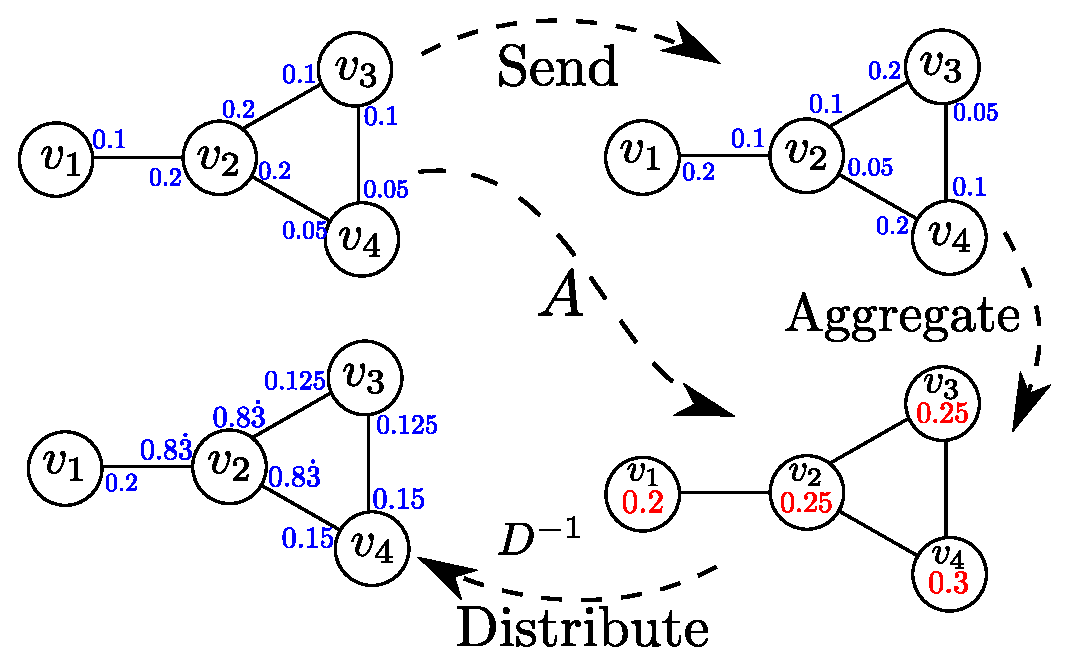
\includegraphics[scale=0.65]{WT.eps}
    \caption{The action of $\mW_G^T$ on the vector $\vx = ({\color{blue}0.1},{\color{blue}0.6},{\color{blue}0.2},{\color{blue}0.1})$.}
    \label{fig:Wt}
\end{figure}

\paragraph{Hilbert Space Interpretation}
One can think of the $\vx$ vectors as living in the Hilbert space with inner product $\langle\cdot ,\cdot\rangle_{\mD}: \R^V \to \R$ given by:
\[
    \langle \vx,\vy \rangle_D = \vx^T\mD\vy
\]
And similarly the $\vp$ vectors live in the dual space with inner product: $\langle \cdot,\cdot\rangle_{\mD^{-1}}: \R^V \to \R$ given by:
\[
    \langle \vp,\vq \rangle_{\mD^{-1}} = \vp^T\mD^{-1}\vq
\]
for any $\vx$ the corresponding vector $\vp$ will equal $\Phi(\vx)$ where $\Phi$ is the isomorphism guaranteed by the Riesz representation theorem\footnote{Read more about it: \url{https://en.wikipedia.org/wiki/Riesz_representation_theorem}}.

\begin{figure}[h]
    \centering
    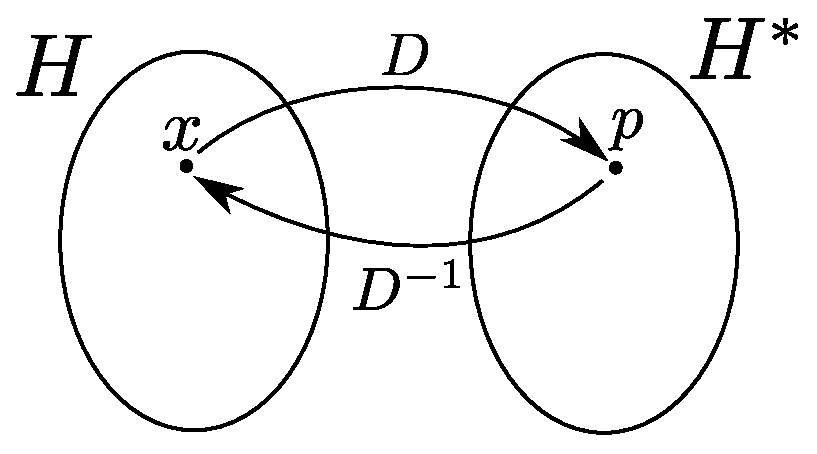
\includegraphics[scale=.75]{HSpaceSGT.eps}
    \caption{Vertex probability vectors $p$ live in the dual Hilbert space to that of edge mass vectors $x$.}
    \label{fig:my_label}
\end{figure}


\section{Notes}

% PACKAGES FOR NETWORK MANIPULATION
% GRAPH LIBRARIES

\paragraph{Graph Storage} How are graphs and matrices stored in computer memory?
Storing the full adjacency matrix requires $O(n^2)$ memory while the graph might only have very few edges. At the same time, queries and operations on the edges can be performed very fast, mostly in O(1) time. When the graph is sparse -- i.e. $|E| = O(m)$, an adjacency list representation may be preferred, even though some operations may be slightly slower.  For a discussion, see:\\ \url{http://en.wikipedia.org/wiki/Graph_\%28abstract_data_type\%29#Representations} \\
Similarly, for matrices, different formats can be used according to whether the matrix is dense or sparse. For instance, you can have a look here:\\
\url{http://netlib.org/linalg/html_templates/node90.html}\\
The compressed column storage used by MATLAB can be thought of as a particular implementation of the adjacency list idea.

\bibliography{bib.bib}
\bibliographystyle{alpha}




\end{document}


%%%%%%%%%%%%%%% TODO:

%%% COURANT-FISHER IN EIGENVALUE PERTURBATION/CHARACTERIZATION

%%% SVD ONLY AS EXERCISE - YES IN SGT, NEED MORE IN LA COURSE

%%%% EXERCISES:
% APPLICATION TO PROVING SVD : YES
% PROVING SPECTRAL DECOMPOSITION OF NORMAL MATRICES: YES
% RANK-k UPDATES AND INTERLACING EIGENVALUES: IN EIGENVALUES PERTRUBATION LECTURE
